\documentclass{beamer}
\usetheme{Madrid}
\usepackage{multimedia}
\usepackage{hyperref}
\hypersetup{
    colorlinks=true,
    linkcolor=blue,
    filecolor=magenta,      
    urlcolor=cyan,
    pdftitle={Overleaf Example},
    pdfpagemode=FullScreen,
    }
\title{Pedistrian dynamics project}
\author{by Amr Elsayed}
\centering
\date{\today}
\begin{document}
\maketitle

\begin{frame}{Content}
\begin{itemize}
\item Motivation
\item parameters used in simulation 
\item Two scenarios used  
\item Simulation of the scenarios
\item simulation data
\item Analysis of the exits data
\item Challenges of the project
\end{itemize}
\end{frame}

\begin{frame}{Motivation}
The aim of this project is to create, simulate and analyze different evacuation
scenarios of the first floor of building HC.
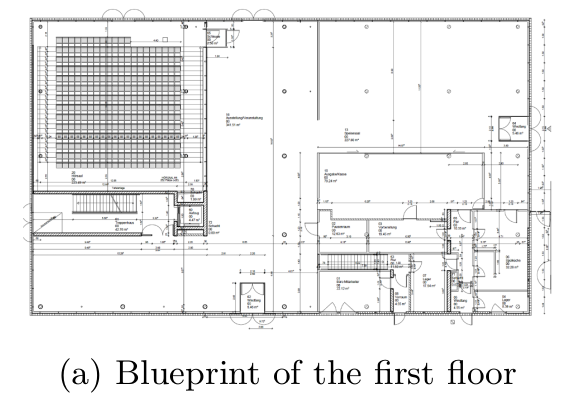
\includegraphics[height=6.8cm]{blueprint.png}
\end{frame}

\begin{frame}{Parameters used in simulation}
\begin{itemize}
\item agents distribution
\begin{itemize}
    \item minimum number of agents used in the simulation are 250
    \item maximum number of agents used in the simulation are 500
\end{itemize}
\item operational model (Tordeux2015)
\begin{itemize}
    \item Model used is a Velocity-based model
    \item The model consists of two components: a direction sub-model that combines individual desired moving direction and neighbor's influence to imitate the process of navigating in a two-dimensional space, and an intrinsically collision-free speed sub-model which controls the speed of the agents with respect to the distance to their neighbors. 
\end{itemize}
\end{itemize}
\end{frame}

\begin{frame}{Two scenarios}
  \framesubtitle{First Scenario:}
  In this scenario, All the doors is open the whole time.
  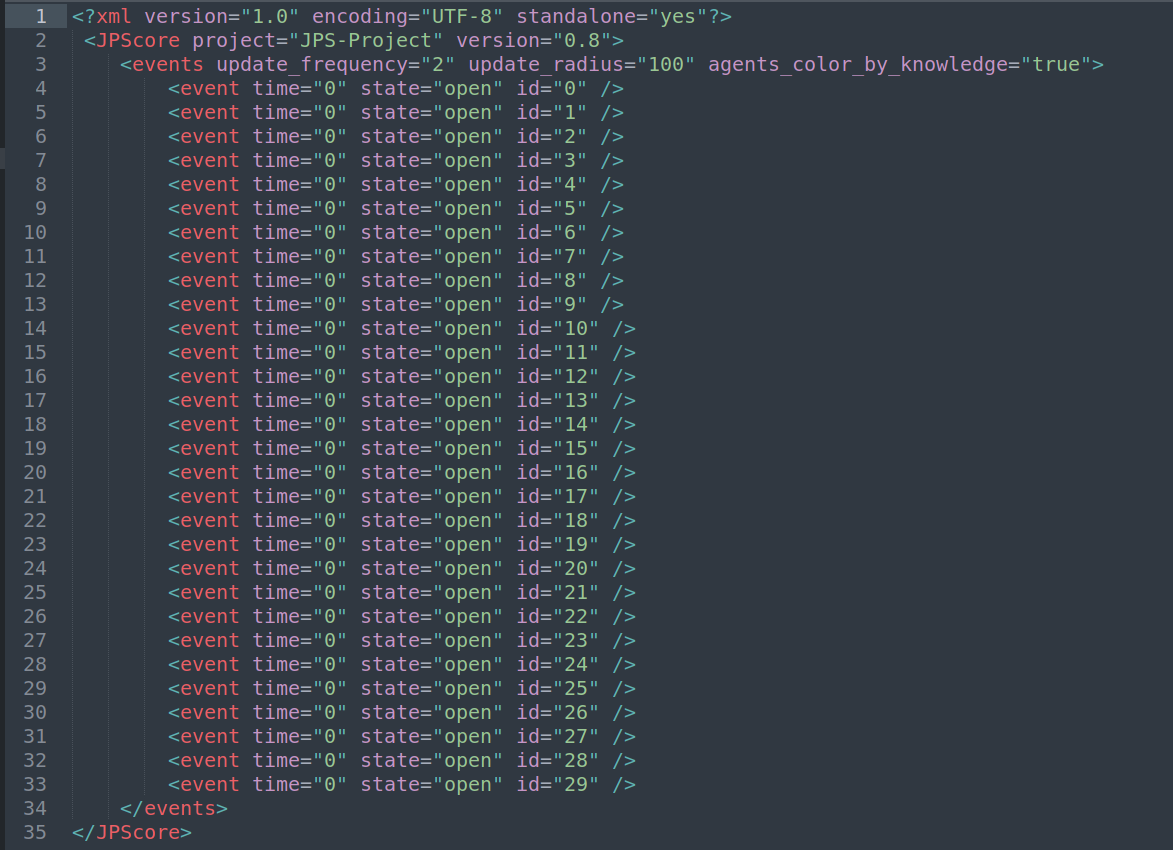
\includegraphics[height=6.5cm]{1st_scenario.png}
\end{frame}

\begin{frame}{Basic two scenarios}
  \framesubtitle{Second Scenario:}
  In this one, I closed specific doors after 10 secs (mainly the offices and kitchen) and the Mensa after 25 secs
  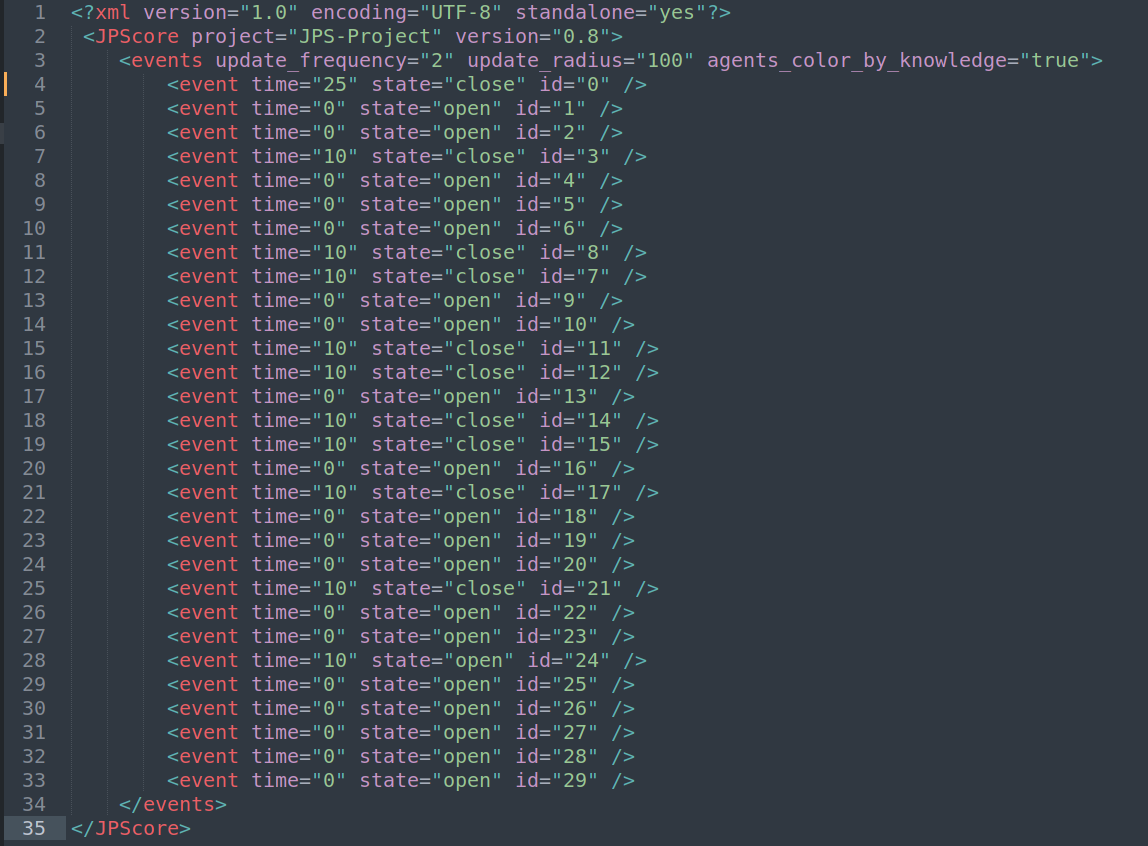
\includegraphics[height=6.5cm]{2nd_scenario.png}
\end{frame}

\begin{frame}
\frametitle{Simulations}
 
\begin{block}{Constant values}
I used the same values in every simulation of:
\begin{itemize}
    \item Distribution of agents (seed)
    \item Operational method
    \item The geometry
\end{itemize}
\end{block}
 
\begin{block}{variable values}
the variables in the simulations are:
\begin{itemize}
    \item number of agents 
    \item changing the goal of the agents
\end{itemize}
\end{block}
\end{frame}

\begin{frame}
\frametitle{First Simulation}
\raggedright
Consider that there is lecture in the main lecture hall (300 agent)and Mensa is fairly busy (100 agent). The evacuation took 82 seconds.
\centering
  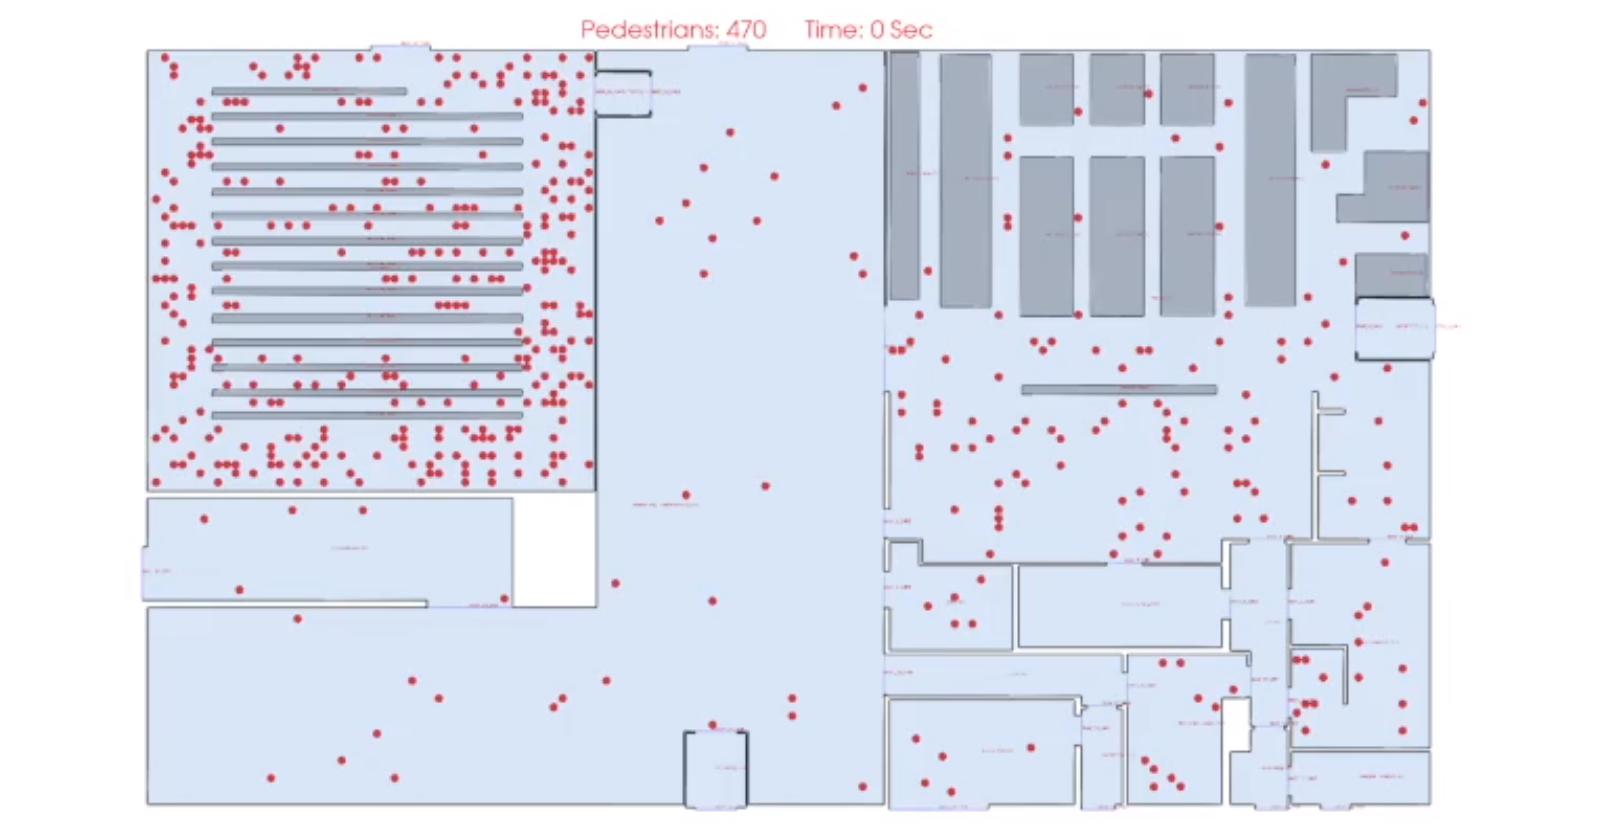
\includegraphics[height=6cm]{01_simulation_start.png}
\end{frame}

\begin{frame}
\frametitle{Analysis of the exits data}
\raggedright
from this graph between the cumulative number of agents \& time, that only the lecture hall taking around 20 seconds more.
\centering
  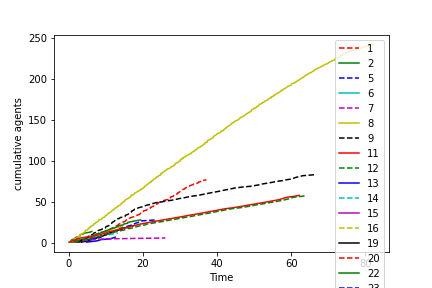
\includegraphics[height=6.5cm]{results_crowd_01.png}
\end{frame}

\begin{frame}
\frametitle{Second Simulation}
\raggedright
Consider that there is no lecture in the main lecture hall (30 agent)and Mensa is crowded (150 agent). The evacuation took 50 seconds.
\centering
  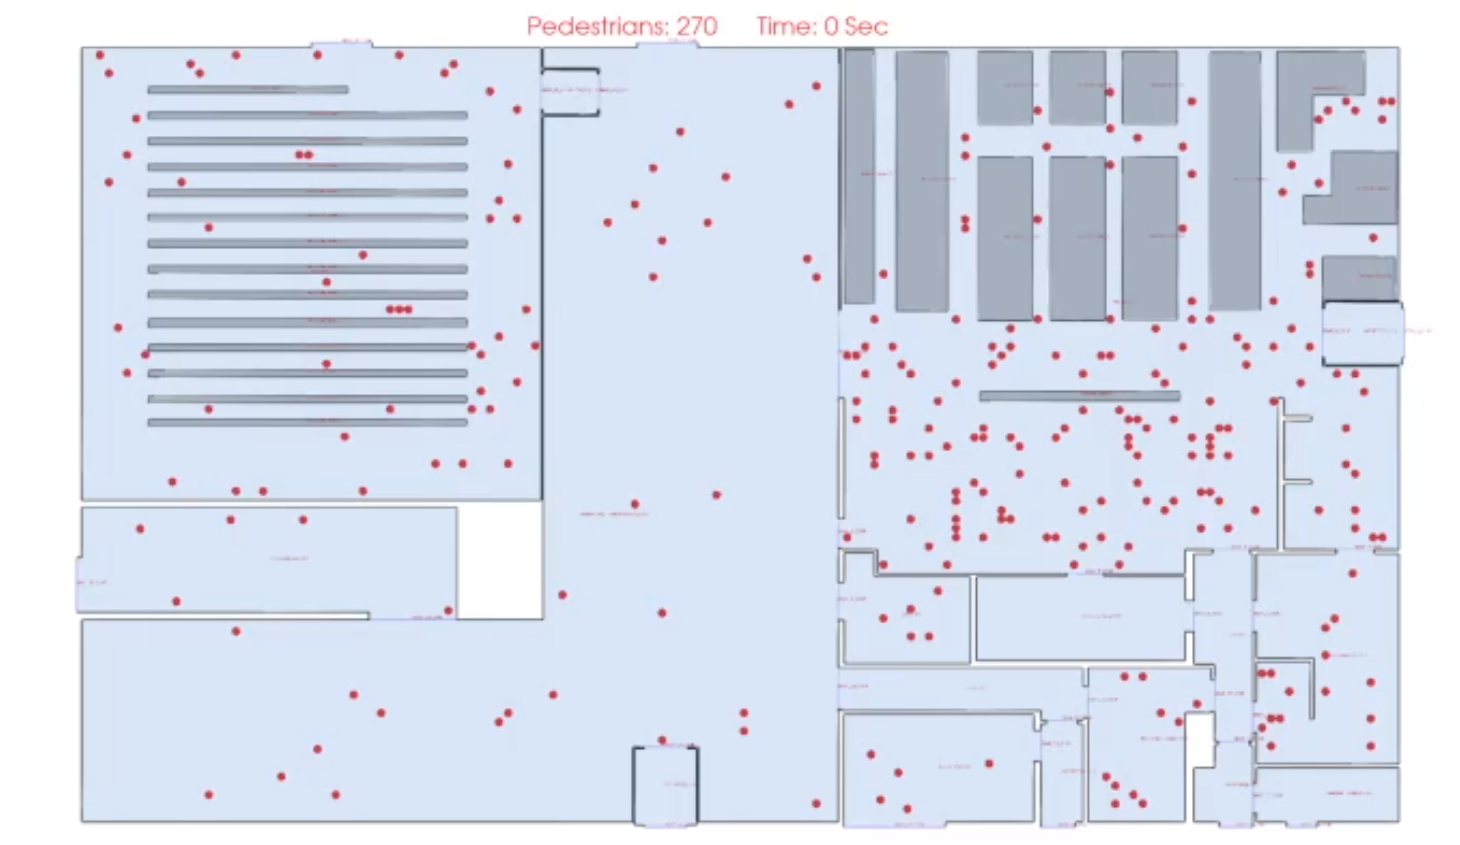
\includegraphics[height=6.5cm]{02_simulation_start.png}
\end{frame}

\begin{frame}
\frametitle{Analysis of the exits data}
\raggedright
in this case the Mensa evacuation taking around 20 more seconds than the other rooms. \\

\centering
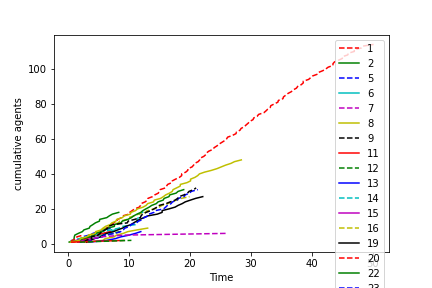
\includegraphics[height=6.5cm]{results_without_lecture_02.png}
\end{frame}

\begin{frame}
\frametitle{Goal}
\raggedright
from the first two simulations, we found that only one room affecting the whole simulation time. \\
As a solution, we had to distribute the agents on the two doors available in the room to decrease the evacuation time and avoid the bottleneck near the exit door. \\
\centering
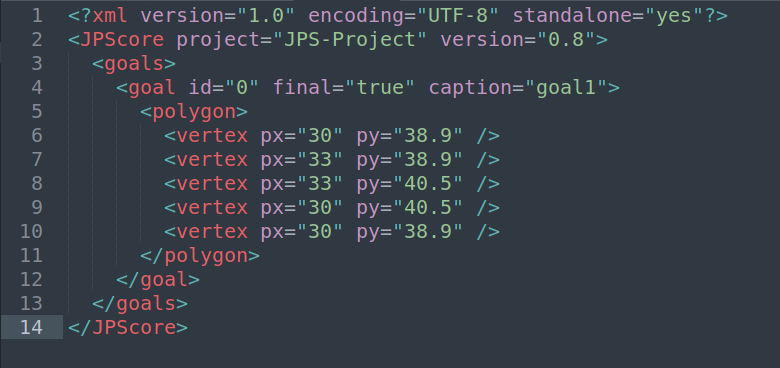
\includegraphics[height=5cm]{goal.png}
\end{frame}

\begin{frame}
\frametitle{Third Simulation}
\raggedright
Its similar to the first simulation but this time with two groups in the lecture hall (100 and 200 agents). to use the doors available in the lecture room.it took 86 seconds.
\\
\centering
 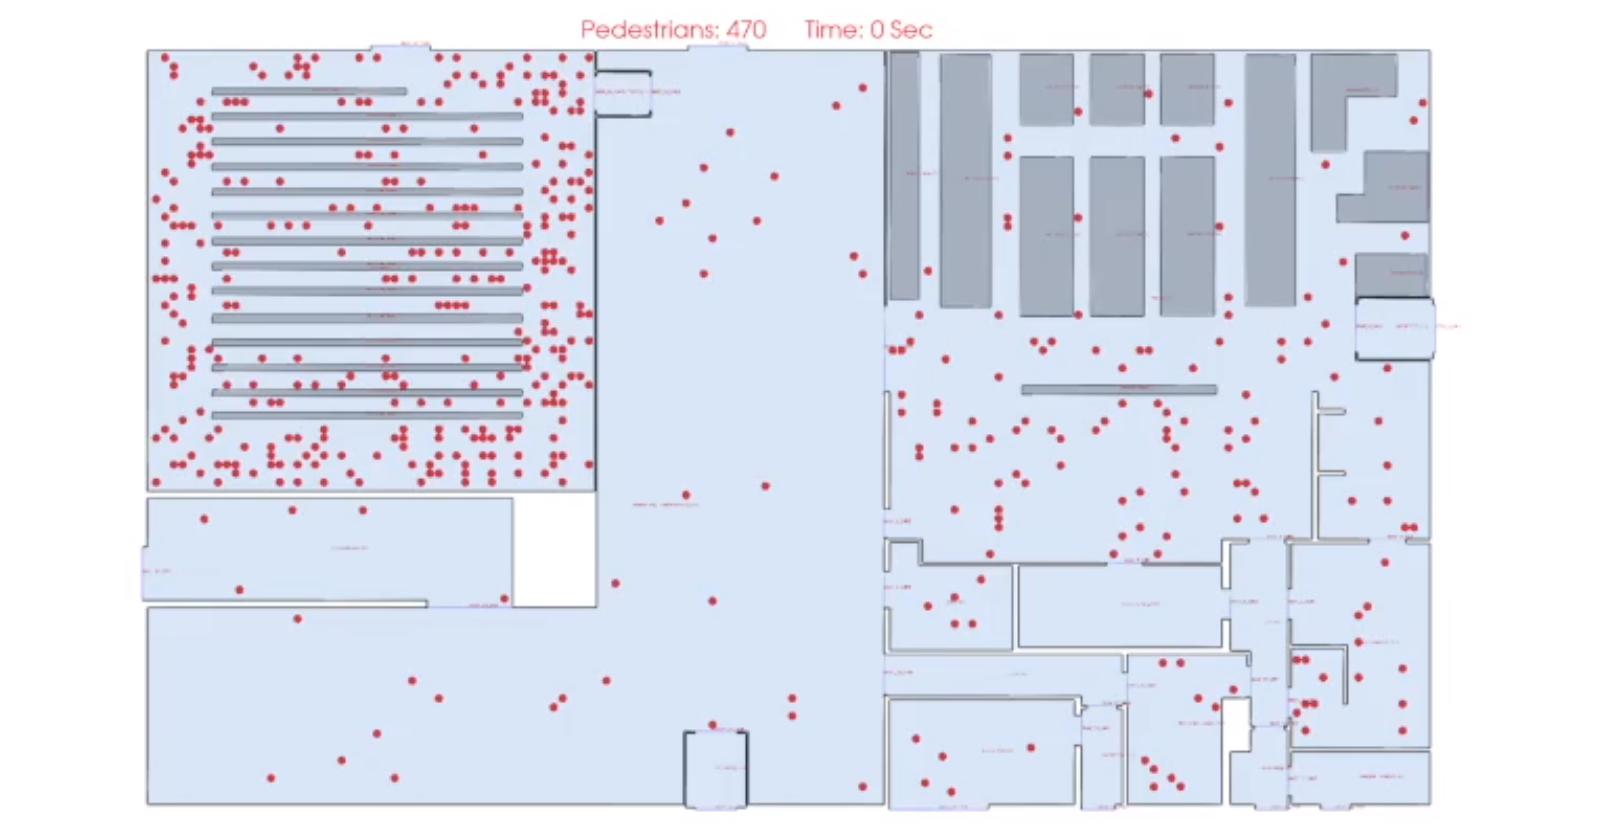
\includegraphics[height=6cm]{01_simulation_start.png}
\end{frame}

\begin{frame}
\frametitle{Analysis of the exits data}
\raggedright
it took almost the same time, but more distributed on the exit doors 
\vspace{1em}
\centering
  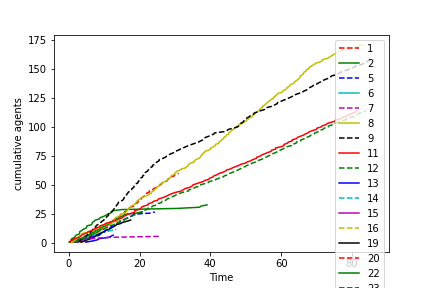
\includegraphics[height=6.5cm]{results_goal_06.png}
\end{frame}

\begin{frame}
\frametitle{Fourth Simulation}
\raggedright
its similar to the Second simulation but this time with two groups in the Mensa (100 agents and 50 agents). to use the doors available in the lecture room.
\centering
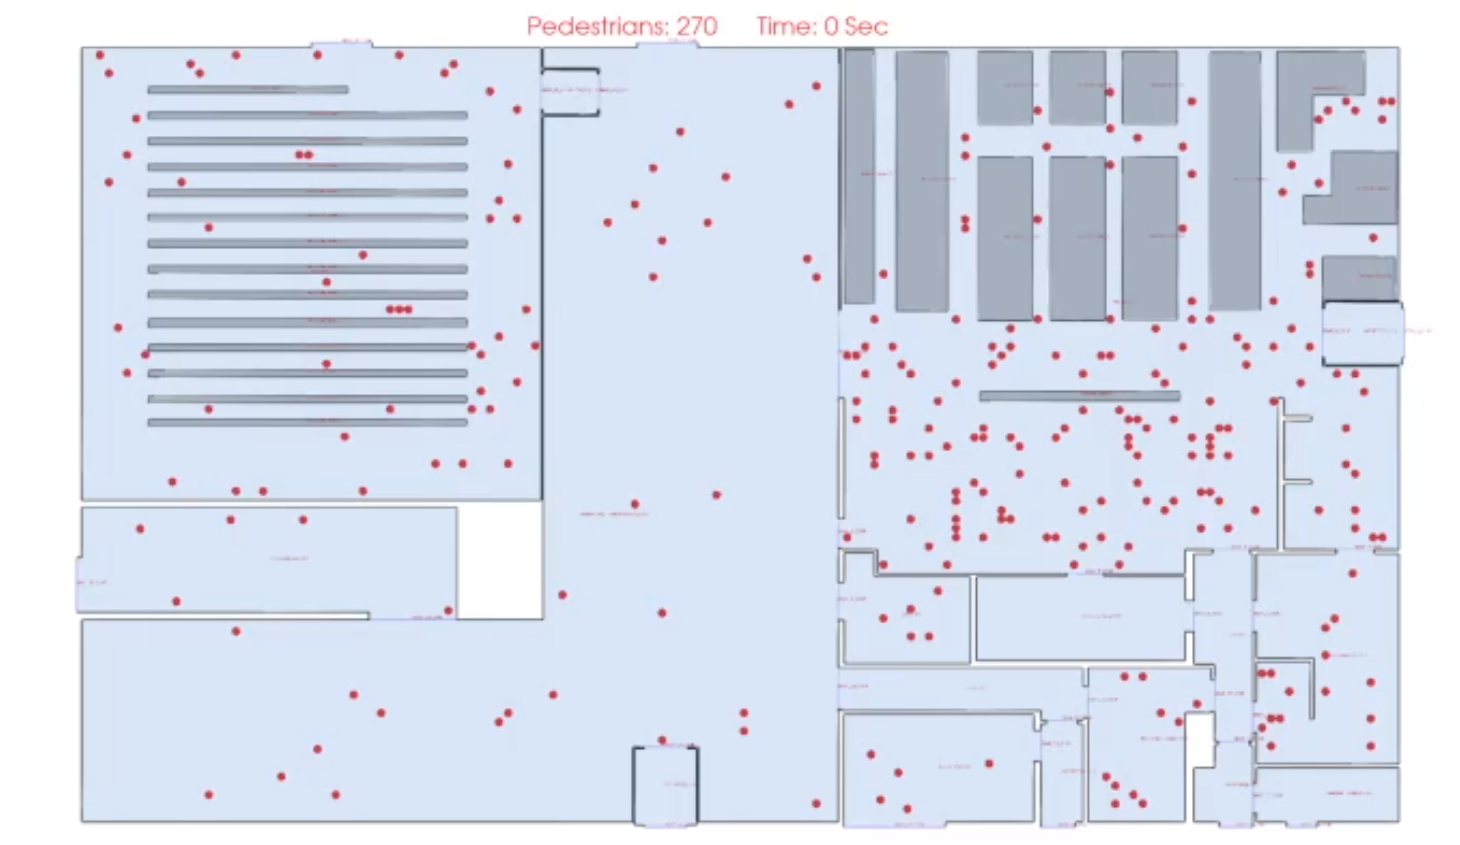
\includegraphics[height=6.5cm]{02_simulation_start.png}
\end{frame}

\begin{frame}
\frametitle{Fourth Simulation}
\centering
Let's see the video
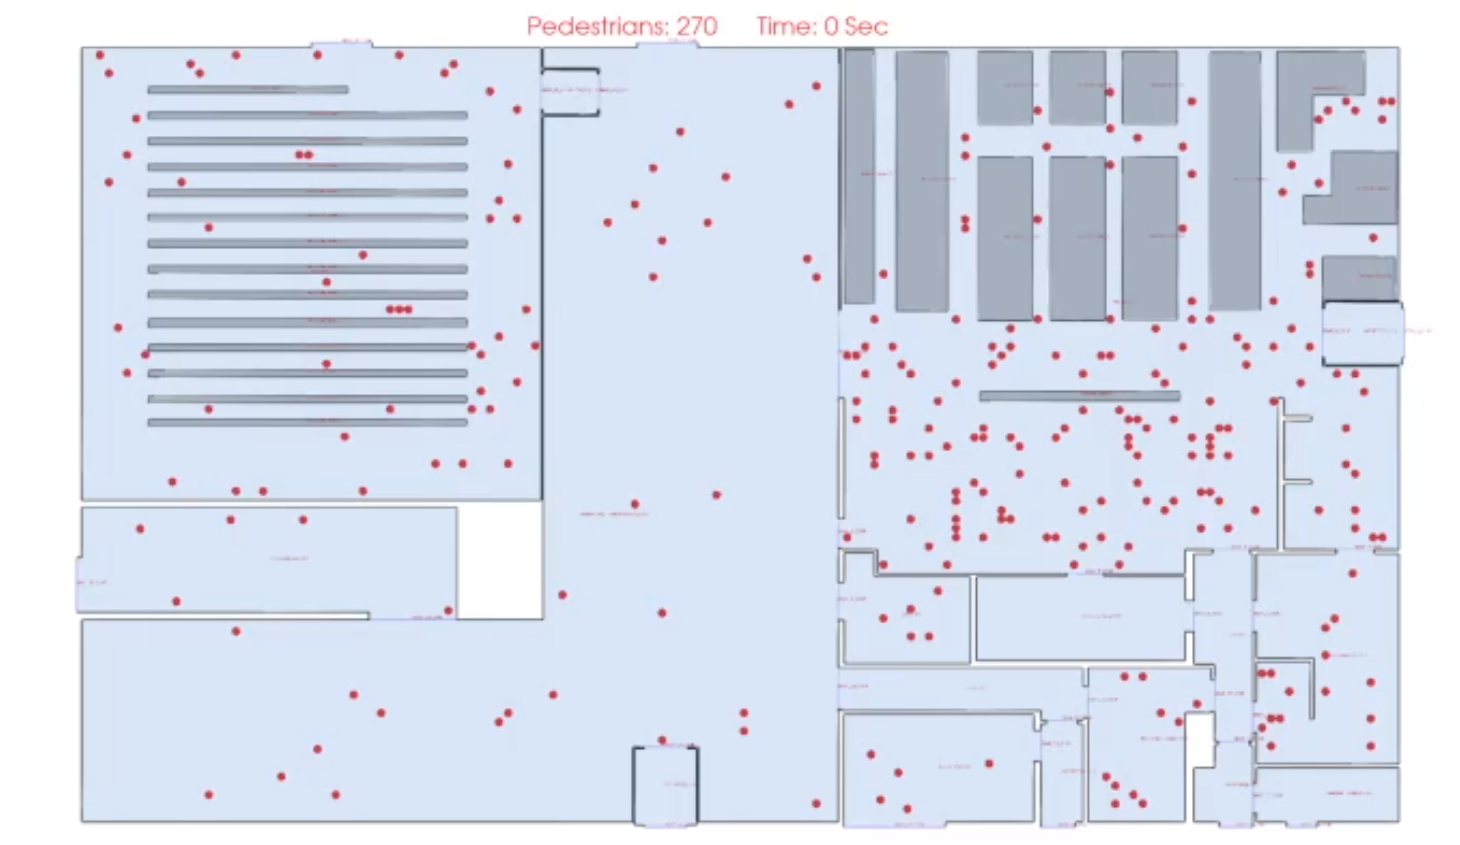
\includegraphics[height=6.5cm]{02_simulation_start.png}
\end{frame}

\begin{frame}
\frametitle{Analysis of the exits data}

\centering
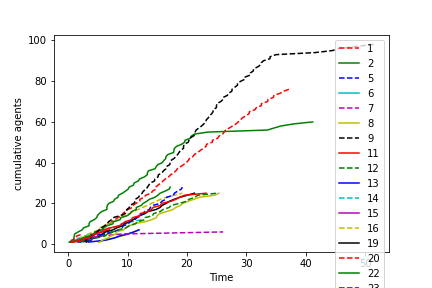
\includegraphics[height=6.5cm]{results_without_lecture_goal_05.png}
\end{frame}

\begin{frame}
\frametitle{GitHub link}
\href{https://github.com/AmrElsayed14/pedestrian_dynamics_jpscore_project.git}{Repository link}

\end{frame}

\begin{frame}
\huge{\centerline{Thanks!}}
\end{frame}

\end{document}
